% !TeX root = ../main.tex
\section{Discussion: look-ahead as a rescue, not an upgrade}
\label{sec:discussion}

\S\ref{sec:mechanism} explains why look-ahead does nothing in generations~2 and~3, but not why
it did something in generation~1. The two must be reconciled by something that differs between
the settings. This section proposes a candidate that is measurable in all three, then says
plainly how much confidence it deserves.

\subsection{The candidate: how well the myopic baseline learns}
The three generations differ in a way that has nothing to do with look-ahead and is visible in
the trajectories of Figure~\ref{fig:trajectories}: \textbf{how much the $\K{=}0$ arm learns on
its own}. On the common grader:

\begin{itemize}\itemsep2pt
  \item \textbf{Generation 1}: base $3.865$, myopic arm after 7 iterations $3.887$. A gain of
  $+0.023$ --- inside grader noise. The one-step reward is essentially inert.
  \item \textbf{Generation 2}: base $2.378$, myopic arms after 5 iterations $2.596$--$2.770$.
  Gains of $+0.22$ to $+0.39$. The one-step reward works.
  \item \textbf{Generation 3}: base $3.008$, myopic arm after 8 iterations $4.221$. A gain of
  $+1.212$. The one-step reward works very well.
\end{itemize}

The ordering is the exact inverse of look-ahead's measured benefit: large where the myopic arm
is inert, absent where it works, negative where it works best.
Figure~\ref{fig:moderator} plots this across the five training arms for which both quantities
exist. The association is $r = -0.72$ ($p = 0.17$) against the myopic arm's per-iteration
slope and $r = -0.84$ ($p = 0.08$) against its total gain.

\begin{figure}[t]
\centering
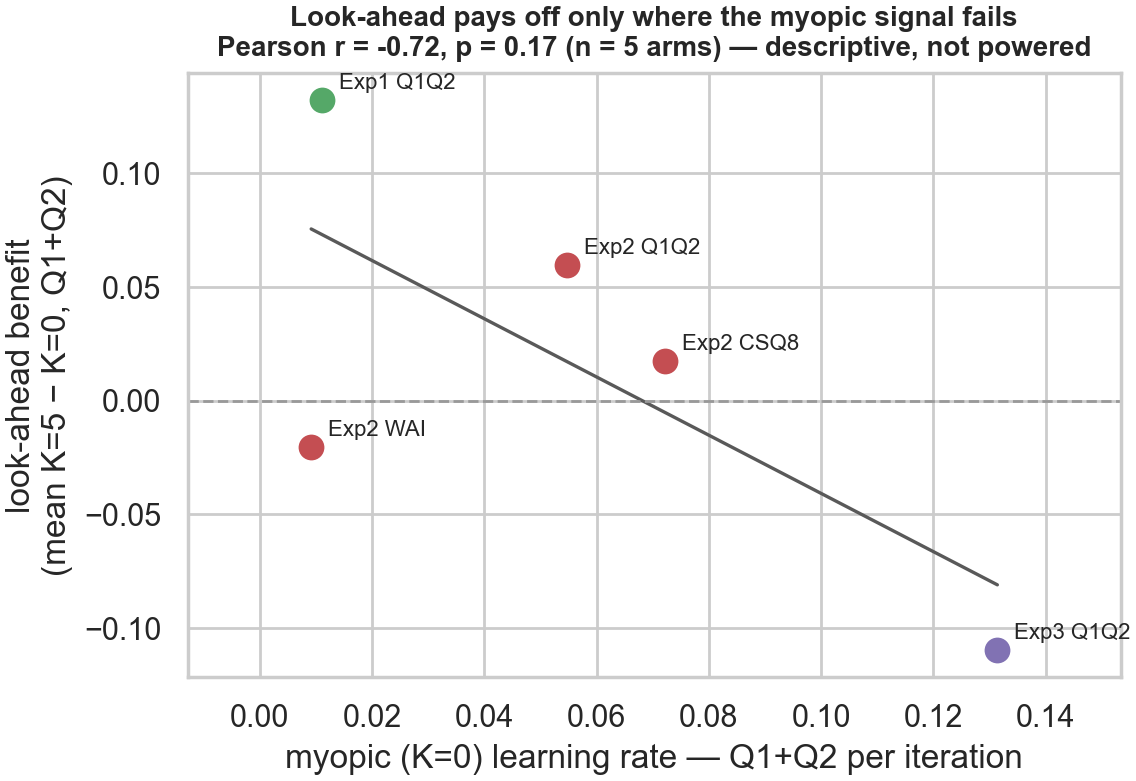
\includegraphics[width=0.72\linewidth]{figures/fig2_moderator.png}
\caption{Look-ahead's measured benefit against how fast the myopic ($\K{=}0$) arm learns, one
point per training arm. Oriented so positive = look-ahead helped. The trend runs the predicted
way, but $n = 5$ and the Exp2/WAI-SR arm sits against it; this is an interpretation, not a
result.}
\label{fig:moderator}
\end{figure}

\subsection{Why this is only an interpretation}
The correlation is not significant, $n = 5$ arms is far too few, and one arm contradicts it
outright: generation~2's WAI-SR arm has a myopic slope as low as generation~1's ($+0.009$
versus $+0.011$) yet shows no look-ahead benefit at all ($-0.020$, i.e.\ slightly negative). If
the moderator were the whole story that arm should have behaved like generation~1 and it did
not. Rank correlations are correspondingly weaker (Spearman $-0.40$ and $-0.60$). We therefore
present this as the reading most consistent with the evidence, not as a finding.

It is worth being explicit about what would test it properly, since nothing here does: hold
everything fixed and vary only the quality of the myopic signal --- for instance by degrading
the oracle, or by varying the minimum-context filter that controls how much conversation the
short reward sees --- and check whether look-ahead's benefit tracks it within a single
generation. That is a single-generation experiment and would be the natural next step.

\subsection{Why the reading is nonetheless attractive}
Three things recommend it.

First, it is consistent with the mechanism. \S\ref{sec:mechanism} finds that look-ahead
rescales the reward without adding information. A rescaling is worth something when the signal
is so weak that the filter $\tau$ is rejecting almost everything and few usable preference
pairs survive; it is worth nothing when the signal is already strong enough to drive learning.
That is precisely a benefit that appears at the bottom of the range and disappears above it.

Second, it explains the direction of the residual in generation~3, where look-ahead is not
merely useless but slightly harmful. Five simulated turns of a 1B policy are five turns of
\emph{noise} appended to each candidate before scoring. When the one-step reward is
uninformative, that trade is worth making; when it is informative, the added variance dilutes
it.

Third, it is what the mechanism section predicts for the confounded factors we cannot separate.
A 7B policy paired with a weak GPT-3.5 grader on cooperative patients is a setting where the
one-step signal has little to say; a 1B policy against a stronger grader and harder patients,
with a minimum-context filter deliberately tuned so that training cuts are long enough to be
informative, is a setting where it has a lot to say. We cannot attribute the reversal to model
size, grader strength or patient difficulty individually (\S\ref{sec:limitations}) --- but all
three moved in the direction that strengthens the myopic signal, and look-ahead's benefit moved
inversely.

\subsection{Practical guidance}
For anyone considering look-ahead simulation in a similar loop, the chapter suggests a cheap
decision procedure that does not require running the expensive arm to completion:

\begin{enumerate}\itemsep2pt
  \item \textbf{Run the myopic arm first.} It is several times cheaper per iteration.
  \item \textbf{Check whether it learns.} If it climbs steadily away from the untrained base,
  the evidence here says look-ahead will not add to it, and may cost a little.
  \item \textbf{Only if it stalls is look-ahead indicated}, and then as a diagnosis that the
  one-step reward is too weak --- for which cheaper remedies exist (a longer minimum context, a
  better rubric, a stronger grader) and should be tried first.
  \item \textbf{Never evaluate the lever best-versus-best.} Compare at matched iteration counts,
  paired on whatever unit dominates the variance --- here, the simulated patient. In
  generation~1 that change alone moved the apparent effect substantially
  (\S\ref{sec:gen1}).
\end{enumerate}

\subsection{On reporting a non-replication of one's own result}
The finding in \S\ref{sec:gen3} contradicts the headline of \citet{baruch2025pto}. Three things
seem worth recording about how that came out.

The original result was not wrong about its own data. Re-analysed with a stricter test and
re-graded with a stronger oracle, generation~1's look-ahead advantage is still there
(\S\ref{sec:gen1}). What was wrong was its scope: a result obtained in one setting was
described as a property of the method.

The two cheap escape hatches were both available and neither worked. It would have been
comfortable to conclude that the original analysis was underpowered, or that the old grader was
fooled. Testing both --- and finding that the paired re-analysis \emph{strengthens} the original
effect and the modern grader \emph{reproduces} it --- is what makes the reversal a real
scientific observation rather than a methodological correction.

The conditional version is more useful than the unconditional one. ``Look-ahead improves
goal-oriented dialogue training'' supports no decision, because it does not say when to pay for
it. ``Look-ahead rescues a failing one-step reward and otherwise wastes several times the
compute'' supports the procedure above. The negative result is the more actionable of the two.
